\setcounter{chapter}{6}
\chapter{Modeling Trends}
{\small \textit{Chapter Preview}. This chapter begins our study of
time series data by introducing techniques to account for major
patterns, or trends, in data that evolve over time. The focus is on
how regression techniques developed in earlier chapters can be used
to model trends. Further, new techniques, such differencing data,
allow us to naturally introduce a random walk, an important model of
efficient financial markets.}


\section{Introduction}

\subsubsection*{Time Series and Stochastic Processes}

Business firms are not defined by physical structures such as the
solid stone bank building that symbolizes financial security. Nor
are businesses defined by space alien invader toys that they
manufacture for children. Business firms are comprised of several
complex, interrelated processes. A \emph{process} is a series of
actions or operations that lead to a particular end.

Processes are not only the building blocks of businesses, they also
provide the foundations for our everyday lives. We may go to work or
school every day, practice martial arts or study statistics. These
are regular sequences of activities that define us. In this text,
our interest is in modeling \index{time series terms and
concepts!stochastic process} \emph{stochastic processes}, defined to
be ordered collections of random variables, that quantify a process
of interest.

\marginparjed{A time series is a single measurement of a process
that yields a variable over time, denoted by $y_1,...,y_T$.}

Some processes evolve over time, such as daily trips to work or
school and the quarterly earnings of a firm. We use the term
\emph{longitudinal data} for measurements of a process that evolves
over time.\index{time series terms and concepts!longitudinal data} A
single measurement of a process yields a variable over time, denoted
by $y_1,...,y_T,$ and referred to as a \emph{time series}.
\index{time series terms and concepts!time series}In this portion of
the text, we follow common practice and use $T$ to denote the number
of observations available (instead of $n$). Chapter 10 will describe
another type of longitudinal data where we examine a cross-section
of entities, such as firms, and examine their evolution over time.
This type of data is also known as \emph{panel data}.

Collections of random variables may be based on orderings other than time.
For example, hurricane claim damages are recorded at the place where the
damage has occurred and thus are ordered spatially. As another example,
evaluation of an oil-drilling project requires taking samples of the earth
at various longitudes, latitudes and depths. This yields observations
ordered by the three dimensions of space but not time. As yet another
example, the study of holes in the ozone layer requires taking atmospheric
measurements. Because the interest is in the trend of ozone depletion, the
measurements are taken at various longitudes, latitudes, heights and time.
Although we consider only processes ordered by time, in other studies of
longitudinal data you may see alternatives orderings. Data that are not
ordered are called \emph{cross-sectional}.

\marginparjed{Cross-sectional data are not ordered by time.}

\subsubsection*{Time Series versus Causal Models}\index{time series models!causal}

Regression methods can be used to summarize many time series data
sets. However, simply using regression techniques without
establishing an appropriate context can be disastrous. This concept
is reinforced by an example based on Granger and Newbold's (1974)
work.

\linejed

\textbf{Example: Spurious Regression.} Let $\{\varepsilon_{x,t}\}$ and $%
\{\varepsilon_{y,t}\}$\ be two independent sequences, each of which
also has a standard normal distribution. From these, recursively
construct the variables $x_t = 0.5 + x_{t-1} + \varepsilon_{x,t}$
and $y_t = 0.5 + y_{t-1} + \varepsilon_{y,t}$, using the initial
conditions $x_0=y_0=0$. (In Section 7.3, we will identify $x_t$\ and
$y_t$\ as random walk models.) Figure \ref{F7:SpurCorr} shows a
realization of \{$x_t$\} and \{$y_t$\}, generated for $T=50$
observations using simulation. The left-hand panel shows the growth
of each series over time - the increasing nature is due to the
addition of 0.5 at each time point. The right-hand panel shows a
strong relationship between \{$x_t$\} and \{$y_t$\} - the
correlation between these two series turns out to be 0.92. This is
despite the fact that the two series were generated
\emph{independently. }Their apparent relationship, said to be
\emph{spurious}, is because both are related to the growth over
time.


\begin{figure}[htp]
  \begin{center}
    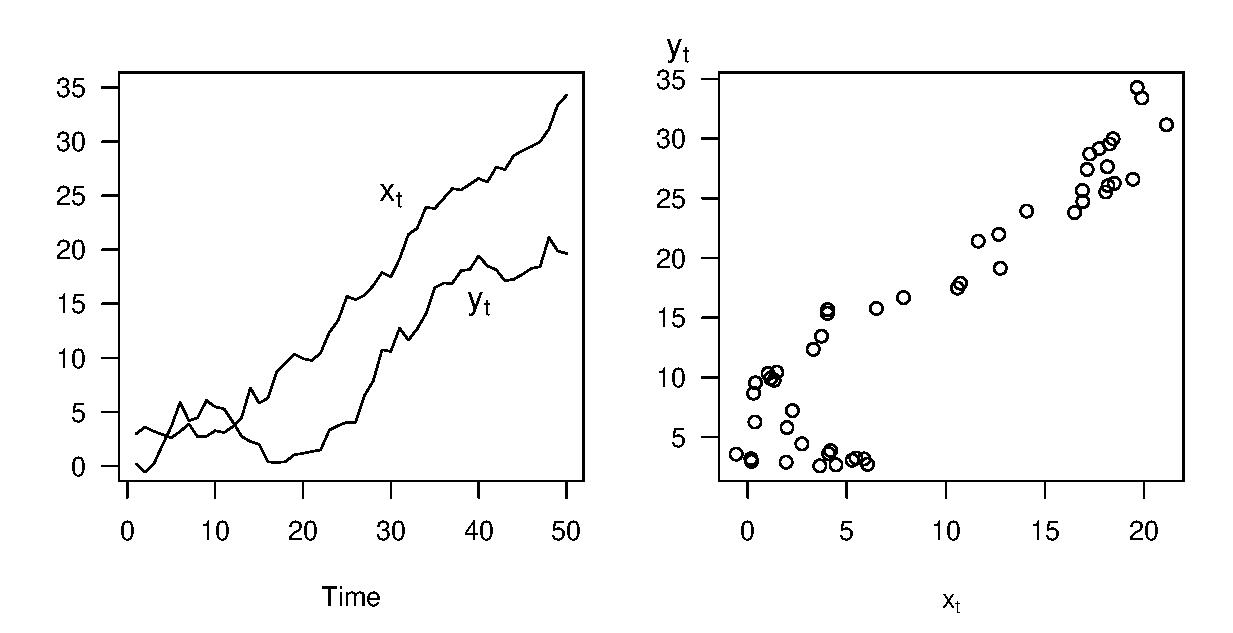
\includegraphics[width=1\textwidth]{Chapter7Trend/Figure71SpurCorr.eps}
    \caption{\label{F7:SpurCorr} \small Spurious
Regressions. The left-hand panel shows two time series that are
increasing over time. The right-hand panel shows a scatter plot of
the two series, suggesting a positive relationship between the two.
The relationship is spurious in the sense that both series are
driven by growth over time, not their positive dependence on one
another.}
  \end{center}
\end{figure}

\linejed

In a longitudinal context, regression models of the form%
\begin{equation*}
y_t = \beta_0 + \beta_1 x_t + \varepsilon_t
\end{equation*}
are known as \emph{causal models}. Causal models are regularly
employed in econometrics, where it is assumed that economic theory
provides the information needed to specify the causal relationship
($x$ ``causes'' $y$). In contrast, statistical models can only
validate empirical relationships (``correlation, not causation'').
In the spurious regression example, both variables evolve over time
and so a model of how one variable influences another needs to
account for time patterns of both the left- and right-hand side
variables. Specifying causal models for actuarial applications can
be difficult for this reason - time series patterns in the
explanatory variables may mask or induce a significant relationship
with the dependent variable. In contrast, regression modeling can be
readily applied when explanatory variables are simply functions of
time, the topic of the next section. This is because functions of
time are deterministic and so will not exhibit time series patterns.

\marginparjed{Regression models can be readily applied when
explanatory variables are functions of time.}

Causal models also suffer from the drawback that their applications
are limited for forecasting purposes. This is because in order to
make a forecast of a future realization of the series, for example
$y_{T+2}$, one needs to have knowledge (or a good forecast) of
$x_{T+2},$ the value of the explanatory variable at time $T+2$. If
$x$ is a known function of time (as in the next section), then this
is not an issue. Another possibility is to use a lagged value of $x$
such as $y_t = \beta_0 + \beta_1 x_{t-1} + \varepsilon_t,$ so that
one-step predictors are possible (we can use the equation to predict
$y_{T+1}$ because $x_T$ is known at time $T$).

\section{Fitting Trends in Time}\label{S7:Trends}

\subsubsection*{Understanding Patterns over Time}

\marginparjed{A forecast is a prediction of a future value of a time
series.}

\emph{Forecasting} is about predicting future realizations of a time
series. Over the years, analysts have found it convenient to
decompose a series into three types of patterns: trends in time
($T_t$), seasonal ($S_t$), and random, or irregular, patterns
($\varepsilon_t$). A series can then be forecast by extrapolating
each of the three patterns. The trend is that part of a series that
corresponds to a long-term, slow evolution of the series. This is
the most important part for long-range forecasts. The seasonal part
of the series corresponds to aspects that repeat itself
periodically, say over a year. The irregular patterns of a series
are short-term movements that are typically harder to
anticipate.\index{time series terms and concepts!forecast}

Analysts typically combine these patterns in two ways: in an
additive fashion,
\begin{equation}\label{E7:1}
y_t = T_t + S_t + \varepsilon_t,
\end{equation}
or in a multiplicative fashion,
\begin{equation}\label{E7:2}
y_t = T_t \times S_t + \varepsilon_t.
\end{equation}
Models without seasonal components can be readily handled by using
$S_t=0$ for the additive model in equation (\ref{E7:1}) and $S_t=1$
for the multiplicative model in equation (\ref{E7:2}). If the model
is purely multiplicative such that $y_t = T_t \times S_t \times
\varepsilon_t$, then it can be converted to an additive model by
taking logarithms of both sides.

\marginparjed{A plot of $y_t$ versus $t$ is called a time series
plot.}

\index{plots!time series}

It is instructive to see how these three components can be combined
to form a series of interest. Consider the three components in
Figure \ref{F7:LinearTrend}. Under the additive model, the trend,
seasonal and random variation components are combined to form the
series that appears in the lower right-hand panel. A plot of $y_t$
versus $t$ is called a \emph{time series plot}. In time series
plots, the convention is to connect adjacent points using a line to
help us detect patterns over time.

When analyzing data, the graph in the lower right-hand panel is the
first type of plot that we will examine. The goal of the analysis is
to go backwards - that is, we wish to decompose the series into the
three components. Each component can then be forecast which will
provide us with forecasts that are reasonable and easy to interpret.


\begin{figure}[htp]
  \begin{center}
    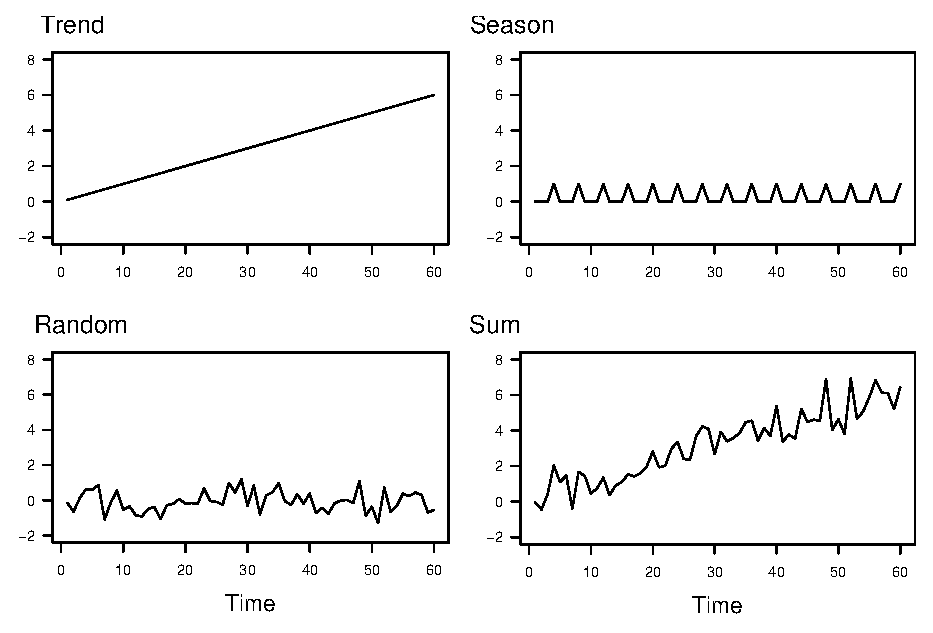
\includegraphics[width=1\textwidth]{Chapter7Trend/Components.eps}
    \caption{\label{F7:LinearTrend} \small Time Series
Plots of Response Components. The linear trend component appears in
the upper left-hand panel, the seasonal trend in the upper right and
the random variation in the lower left. The sum of the three
components appears in the lower right-hand panel.}
  \end{center}
\end{figure}


\subsubsection*{Fitting Trends in Time}

The simplest type of time trend is a complete lack of trend.
Assuming that the observations are identically and independently
distributed (\emph{i.i.d.}), then we could use the model
\begin{equation*}
y_t = \beta_0 + \varepsilon_t.
\end{equation*}
For example, if you are observing a game of chance such as bets
placed on the roll of two dice, then we typically model this as an
i.i.d. series.

\marginparjed{The linear trend in time model is a regression model
with a straight line in time as the regression function.}

Fitting polynomial functions of time is another type of trend that
is easy to interpret and to fit to the data. We begin with a
straight line for our polynomial function of time, yielding the
\emph{linear trend in time model},\index{time series models!linear
trend in time}
\begin{equation}\label{E7:3}
y_t = \beta_0 + \beta_1 t + \varepsilon_t.
\end{equation}
Similarly, regression techniques can be used to fit other functions
that represent trends in time. Equation (\ref{E7:3}) is easily
extended to handle a \emph{quadratic trend in time},\index{time
series models!quadratic trend in time}
\begin{equation*}
y_t = \beta_0 + \beta_1 t + \beta_2 t^2 + \varepsilon_t,
\end{equation*}
or a higher-order polynomial.

\linejed

\empexjed{HKExchange}\index{datasets!Hong Kong exchange rates}

\textbf{Example: Hong Kong Exchange Rates.}\ecaptionjed{Hong Kong
Exchange Rates} For travelers and firms, exchange rates are an
important part of the monetary economy. The exchange rate that we
consider is the number of Hong Kong dollars that one can purchase
for one US dollar. We have $T=502$ daily observations for the period
April 1, 2005 through May 31, 2007 that were obtained from the
Federal Reserve (H10 report). Figure \ref{F7:HKFits} provides a time
series plot of the Hong Kong exchange rate.

\begin{figure}[htp]
  \begin{center}
        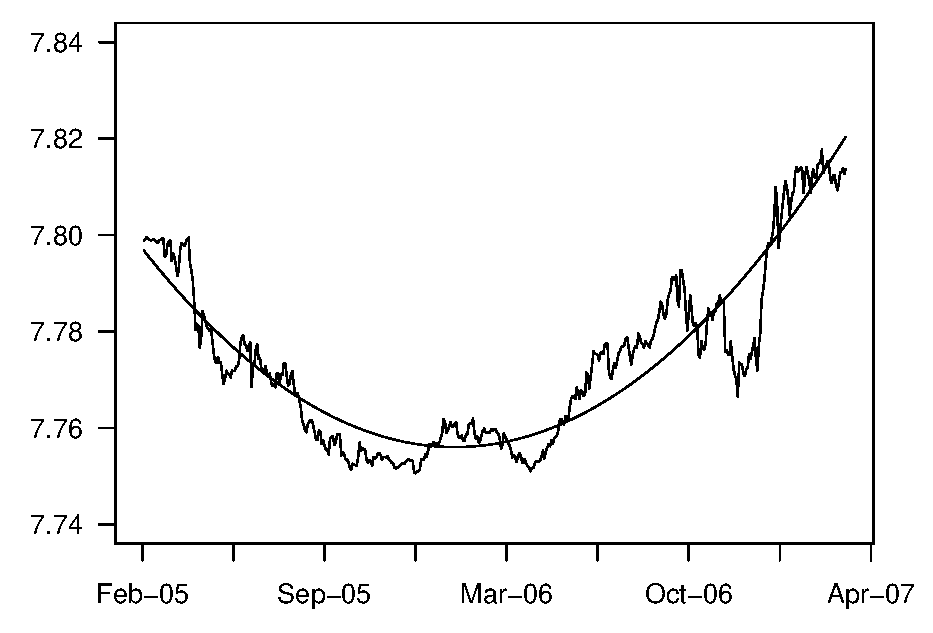
\includegraphics[width=.6\textwidth]{Chapter7Trend/HKFits.eps}
    \caption{\label{F7:HKFits} \small Time Series Plot of Hong Kong
    Exchange Rates with Fitted Values Superimposed. The fitted values are from a regression using a quadratic time trend.
     \emph{Source}: Foreign Exchange Rates (Federal Reserve, H10 report).}
  \end{center}
\end{figure}


Figure \ref{F7:HKFits} shows a clear quadratic trend in the data. To
handle this trend, we use $t=1,...,502$, as an explanatory variable
to indicate the time period. The fitted regression equation turns
out to be:
\begin{equation*}
\begin{tabular}{cccc}
$\widehat{INDEX}_t = $ & $7.797$ & $-3.68\times 10^{-4}t$ &
$+8.269\times
10^{-7}t^2$ \\
{\small $t$-statistics} & {\small (8,531.9)} & {\small (-44.0)} &
{\small (51.2)}
\end{tabular}
.
\end{equation*}
The coefficient of determination is a healthy $R^2=92.9\%$ and the
standard deviation estimate has dropped from $s_{y}=0.0183$ down to
$s=0.0068$ (our residual standard deviation). Figure \ref{F7:HKFits}
shows the relationship between the data and fitted values through
the time series plot of the exchange rate with the fitted values
superimposed. To apply these regression results to the forecasting
problem, suppose that we wanted to predict the exchange rate for
April 1, 2007, or $t=503$. Our prediction is
\begin{equation*}
\widehat{INDEX}_{503} = 7.797 - 3.68 \times 10^{-4}(503) + 8.269
\times 10^{-7}(503)^2 = 7.8208.
\end{equation*}

The overall conclusion is that the regression model using a
quadratic term in time $t$ as an explanatory variable fits the data
well. A close inspection of Figure \ref{F7:HKFits}, however, reveals
that there are patterns in the residuals where the responses are in
some places consistently higher and in other places consistently
lower than the fitted values. These patterns suggest that we can
improve upon the model specification. One way would be to introduce
a higher order polynomial model in time. In Section 7.3, we will
argue that the random walk is an even better model for this data.

\linejed

Other nonlinear functions of time may also be useful. To illustrate,
we might study some measure of interest rates over time ($y_t$) and
be interested in the effect of a change in the economy (such as the
advent of a war). Define $z_t$ to be a binary variable that is zero
before the change occurs and is one during and after the change.
Consider the model,
\begin{equation} \label{E7:4}
y_t = \beta_0 + \beta_1 z_t + \varepsilon_t.
\end{equation}
Thus, using
\begin{equation*}
\mathrm{E~}y_t = \left\{
\begin{array}{ll}
\beta_0 + \beta_1 & if~z_t=1 \\
\beta_0 & if~z_t = 0
\end{array}
\right. ,
\end{equation*}
the parameter $\beta_1$ captures the expected change in interest
rates due to the change in the economy. See Figure
\ref{F7:RegimeSwitch}.


\begin{figure}[htp]
  \begin{center}
    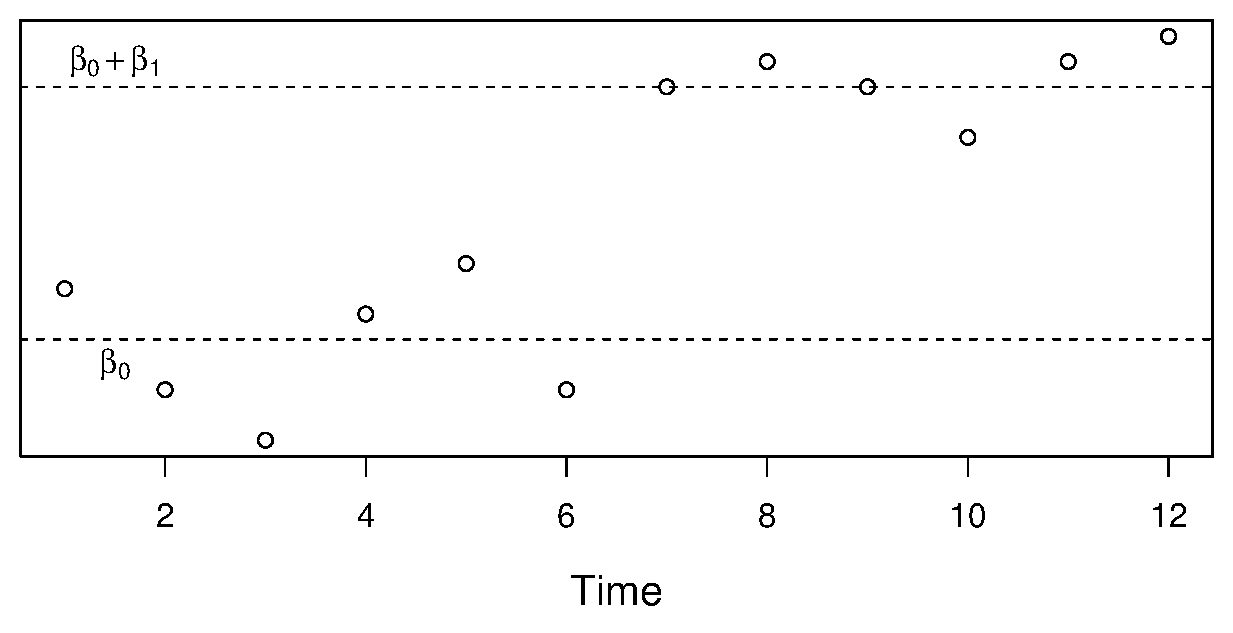
\includegraphics[width=0.6\textwidth]{Chapter7Trend/RegimeSwitch.eps}
    \caption{\label{F7:RegimeSwitch} \small Time
Series Plot of Interest Rates. There is a clear shift in the rates
due to a change in the economy. This shift can be measured using a
regression model with an explanatory variable to indicate the
change.}
  \end{center}
\end{figure}

\linejed

\index{examples!long-term stock returns}

\textbf{Example: Regime-Switching Models of Long-Term Stock
Returns.}\ecaptionjed{Long-Term Stock Returns} With the assumption
of normality, we can write the model in equation (\ref{E7:4}) as
\begin{equation*}
y_t \sim \left\{
\begin{array}{ll}
N(\mu_1, \sigma^2) & t < t_0 \\
N(\mu_2, \sigma^2)& t \geq t_0
\end{array}
\right. ,
\end{equation*}
where $\mu_1 = \beta_0$, $\mu_2 = \beta_0 + \beta_1$ and $t_0$ is
the change point. A \emph{regime-switching} model generalizes this
concept, primarily by assuming that the change point is not known.
Instead, one assumes there exists a transition mechanism that allows
us to shift from one ``regime'' to another with a probability that
is typically estimated from the data. In this model, there is a
finite number of states, or ``regimes.'' Within each regime, a
probabilistic model is specified, such as the (conditionally)
independent normal distribution ($N(\mu_2, \sigma^2)$). One could
also specify an autoregressive or conditionally autoregressive model
that we will define in Chapter 8. Further, there is a conditional
probability of transiting from one state to another (so-called
``Markov'' transition probabilities).

Hardy (2001) introduced regime-switching models to the actuarial
literature where the dependent variable of interest was the
long-term stock market return as measured by  monthly returns on (1)
the Standard and Poor's 500 and the Toronto Stock Exchange 300.
Hardy considered two and three regime models for data over 1956 to
1999, inclusive. Hardy showed how to use the parameter estimates
from the regime-switching model to compute option prices and risk
measures for equity-linked insurance contracts.

\linejed


\subsubsection*{Fitting Seasonal Trends}

Regular periodic behavior is often found in business and economic
data. Because such periodicity is often tied to the climate, these
trends are called \emph{seasonal components}. Seasonal trends can be
modeled using the same techniques as with regular, or aperiodic,
trends. The following example shows how to capture periodic behavior
using seasonal binary variables.\index{time series terms and
concepts!seasonal component}

\linejed

\textbf{Example: Trends in Voting.}\ecaptionjed{Voting Trends} On
any given election day, the number of voters that actually turn out
to voting booths depend on a number of factors: the publicity that
an election race has received, the issues that are debated as part
of the race, other issues facing voters on election day, and
nonpolitical factors, such as the weather. Now, potential political
candidates base their projections of campaign financing, and chances
of winning an election, on forecasts of the number of voters who
will actually participate in an election. Decisions as to whether or
not to participate as a candidate must be made well in advance;
generally, so far in advance that well-known factors such as the
weather on election day can not be used in generating forecasts.

We consider here the number of Wisconsin voters who participated in
statewide elections over the period 1920 through 1990. Although the interest
is in forecasting the actual number of voters, we consider voters as a
percentage of the qualified voting public. Dividing by the qualified voting
public controls for the size of the population of voters; this enhances
comparability between the early and latter parts of the series. Because
mortality trends are relatively stable, reliable projections of the
qualified voting public can be readily attained. Forecasts of the percentage
may then be multiplied by projections of the voting public to obtain
forecasts of the actual voter turnout.

To specify a model, we examine Figure \ref{F7:WiscVotes}, a time
series plot of the voter turnout as a percent of the qualified
voting public. This figure displays the low voter turnout in the
early part of the series, followed by larger turnout in the 1950's
and 1960's, followed by a smaller turnout in the 1980's. This
pattern can be modeled using, for example, a quadratic trend in
time. The figure also displays a much larger turnout in presidential
elections years. This periodic, or seasonal, component can be
modeled using a binary variable. A candidate model is
\begin{equation*}
y_t=\beta_0+\beta_1t+\beta_2t^2+\beta_{3}z_t+\varepsilon _t,
\end{equation*}
where

\begin{equation*}
z_t=\left\{
\begin{array}{ll}
1 & if~\mathrm{presidential\ election\ year} \\
0 & otherwise
\end{array}
\right. .
\end{equation*}
Here, $\beta_{3}z_t$ captures the seasonal component in this model.

Regression was used to fit the model. The fitted model provided a
good fit of the data - the coefficient of determination from the fit
was $R^2=89.6\%.$ Figure \ref{F7:WiscVotes} shows a strong
relationship between the fitted and actual values.

\begin{figure}[htp]
  \begin{center}
    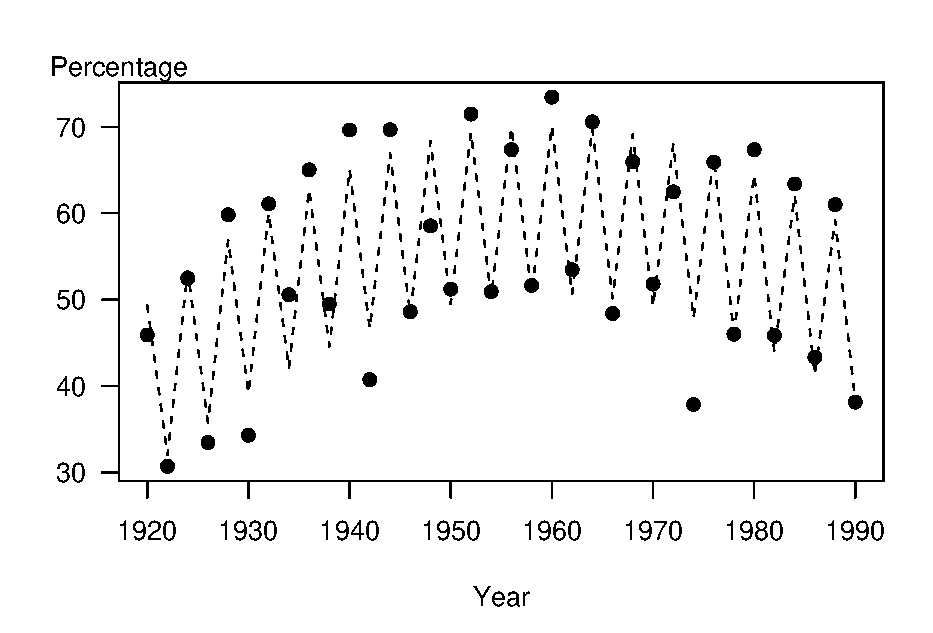
\includegraphics[height=2.5in, width=4.5in]{Chapter7Trend/WiscVotes.eps}
    \caption{\label{F7:WiscVotes} \small Wisconsin
Voters as a Percentage of the Qualified Voting Public, by Year. The
opaque circles represent the actual voting percentages. The dashed
lines represent the fitted trend, using a quadratic trend in time
plus a binary variable to indicate a presidential election year.}
  \end{center}
\end{figure}

\linejed

The voting trend example demonstrates the use of binary variables to
capture seasonal components. Similarly, seasonal effects may be also
be represented using categorical variables, such as
\begin{equation*}
z_t=\left\{
\begin{array}{ll}
1 & if\text{~spring} \\
2 & if\text{~summer} \\
3 & if\text{~fall} \\
4 & if\text{~winter}%
\end{array}%
\right. .
\end{equation*}

Another way of capturing seasonal effects is through the use of
trigonometric functions. Further discussion of the use of trigonometric
functions to handle seasonal components is in Section 9.3.

\marginparjed{Removal of seasonal patterns is known as seasonal
adjustment.}\index{time series terms and concepts!seasonal
adjustment}

Removal of seasonal patterns is known as \emph{seasonal adjustment}.
This strategy is appropriate in public policy situations where
interest centers on interpreting the resulting ``seasonally adjusted
series.'' For example, government agencies typically report
industrial manufacturing revenues in terms of seasonally adjusted
numbers, with the understanding that known holiday and weather
related patterns are accounted for when reporting growth. However,
for most actuarial and risk management applications, the interest is
typically in forecasting the variation of the entire series, not
just the seasonally adjusted portion.

\subsubsection*{Reliability of Time Series Forecasts}

Time series forecasts are sometimes called ``naive'' forecasts. The
adjective ``naive'' is somewhat ironic because many time series
forecasting techniques are technical in nature and complex to
compute. However, these forecasts are based on extrapolating a
single series of observations. Thus, they are naive in the sense
that the forecasts ignore other sources of information that may be
available to the forecaster and users of the forecasts. Despite
ignoring this possibly important information, time series forecasts
are useful in that they provide an objective benchmark that other
forecasts and expert opinions can be compared against.

\marginparjed{Projections should provide a user with a sense of the
reliability of the forecast.}

Projections should provide a user with a sense of the reliability of
the forecast. One way of quantifying this is to provide forecasts
under ``low-intermediate-high'' sets of assumptions. For example, if
we are forecasting the national debt, we might do so under three
scenarios of the future performance of the economy. Alternatively,
we can calculate prediction intervals using many of the models for
forecasting that are discussed in this text. Prediction intervals
provide a measure of reliability that can be interpreted in a
familiar probabilistic sense. Further, by varying the desired level
of confidence, the prediction intervals vary, thus allowing us to
respond to ``what if'' types of questions.

For example, in Figure 21.10 you will find a comparison of
``low-intermediate-high'' projections to prediction intervals for
forecasts of the inflation rate (CPI) used in projecting Social
Security funds. The low-intermediate-high projections are based on a
range of expert opinions and thus reflect variability of the
forecasters. The prediction intervals reflect innovation uncertainty
in the model (assuming that the model is correct). Both ranges give
the user a sense of reliability of the forecasts although in
different ways.

Prediction intervals have the additional advantage in that they
quantify the fact that forecasts become less reliable the further
that we forecast into the future. Even with cross-sectional data, we
saw that the farther away we were from the main part of the data,
the less confident we felt in our predictions. This is also true in
forecasting for longitudinal data. It is important to communicate
this to consumers of forecasts, and prediction intervals are a
convenient way of doing so.

\marginparjed{In forecasting, the primary concern is for the most
recent part of the series.}

In summary, regression analysis using various functions of time as
explanatory variables is a simple yet powerful tool for forecasting
longitudinal data. It does, however, have drawbacks. Because we are
fitting a curve to the entire data set, there is no guarantee that
the fit for the most recent part of the data will be adequate. That
is, for forecasting, the primary concern is for the most recent part
of the series. We know that regression analysis estimates give the
most weight to observations with unusually large explanatory
variables. To illustrate, using a linear trend in time model, this
means giving the most weight to observations at the end and \emph{at
the beginning }of the series. Using a model that gives large weight
to observations at the beginning of the series is viewed with
suspicion by forecasters. This drawback of regression analysis
motivates us to introduce additional forecasting tools. (Section 9.1
develops this point further.)

\section{Stationarity and Random Walk Models}\label{S7:RandomWalk}

A basic concern with processes that evolve over time is the
\emph{stability} of the process. For example: ``Is it taking me
longer to get to work since they put in the new stop light?'' ``Have
quarterly earnings improved since the new CEO took over?'' We
measure processes to improve or manage their performance and to
forecast the future of the process. Because stability is a
fundamental concern, we will work with a special kind of stability
called \emph{stationarity}.\bigskip

\boxedjed

\textbf{Definition.} \ Stationarity is the formal mathematical
concept corresponding to the ``stability'' of a time series of data.
A series is said to be (weakly) stationary if\index{time series
terms and concepts!stationary}

\begin{itemize}
\item the mean $\mathrm{E~}y_t$ does not depend on $t$ and

\item the covariance between $y_{s}$ and $y_t$ depends only on the
difference between time units, $|t-s|.$
\end{itemize}

\end{boxedminipage}

\bigskip

Thus, for example, under weak stationarity $\mathrm{E~}y_{4}=\mathrm{E~}%
y_{8} $ because the means do not depend on time and thus are equal. Further,
$\mathrm{Cov}(y_{4},y_{6})=\mathrm{Cov}(y_{6},y_{8})$, because $y_{4}$ and $%
y_{6}$ are two time units apart, as are $y_{6}$ and $y_{8}$. As
another implication of the second condition, note that $\sigma^2 =
\mathrm{Cov}(y_t, y_t) = \mathrm{Cov}(y_s, y_s) = \sigma^2$. Thus, a
weakly stationary series has a constant mean as well as a constant
variance (homoscedastic). Another type of stationarity known as
\emph{strict, or strong, stationarity} requires that the entire
distribution of $y_t$ be constant over time, not just the mean and
the variance.\index{time series terms and concepts!stationary!weak
stationarity}\index{time series terms and concepts!stationary!strong
stationarity}

\marginparjed{A weakly stationary series has a constant mean as well
as a constant variance (homoscedastic).}\index{homoscedasticity}


\subsubsection*{White Noise}

The link between longitudinal and cross-sectional models can be
established through the notion of a \emph{white noise }process. A
white noise process is a stationary process that displays no
apparent patterns through time. More formally, a white noise process
is simply a series that is \emph{i.i.d.}, identically and
independently distributed. A white noise process is only one type of
stationary process - Chapter 8 will introduce another type, an
autoregressive model.\index{time series models!white noise}


\marginparjed{A white noise process is a stationary process that
displays no apparent patterns through time - it is i.i.d.}

A special feature of the white noise process is that forecasts do
not depend on how far into the future that we wish to forecast.
Suppose that a series of observations, $y_1,...,y_T$, has been
identified as a white noise process. Let $\overline{y}$\ and $s_y$
denote the sample average and standard deviation, respectively. A
forecast of an observation in the future, say $y_{T+l}$, for $l$
lead time units in the future, is $\overline{y}$. Further, a
forecast interval is
\begin{equation}\label{E7:ForecastInterval}
\overline{y}\pm \ t_{T-1,1-\alpha/2} ~ s_y \sqrt{1+\frac{1}{T}}.
\end{equation}
In time series applications, because the sample size $T$ is
typically relatively large, we use the approximate 95\% prediction
interval $ \overline{y} \pm 2 s_y. $ This approximate forecast
interval ignores the parameter uncertainty in using $\overline{y}$\
and $s_y$\ to estimate the mean $\mathrm{E}~y$\ and standard
deviation $\sigma $\ of the series. Instead, it emphasizes the
uncertainty in future realizations of the series (known as
\emph{innovation uncertainty}). Note that this interval does
\emph{not} depend on the choice of $l$, the number of lead units
that we forecast into the future.\index{time series terms and
concepts!innovation uncertainty}


\marginparjed{The white noise model is both the least and the most
important of time series models.}

The white noise model is both the least and the most important of
time series models. It is the least important in the sense that the
model assumes that the observations are unrelated to one another, an
unlikely event for most series of interest. It is the most important
because our modeling efforts are directed towards reducing a series
to a white noise process. In time series analysis, the procedure for
reducing a series to a white noise process is called a
\emph{filter}. After all patterns have been filtered from the data,
the uncertainty is said to be \emph{irreducible}.\index{time series
terms and concepts!filter}\index{time series terms and
concepts!irreducible}

\subsubsection*{Random Walk}

We now introduce the \emph{random walk model}. For this time series
model, we will show how to filter the data simply by taking
differences.\index{time series models!random walk}

To illustrate, suppose that you play a simple game based on the roll
of the two dice. To play the game, you must pay \$7 each time you
roll the dice. You receive the number of dollars corresponding the
sum of the two dice, $c_t^{\ast}$. Let $c_t$ denote your winnings on
each roll, so that $c_t = c_t^{\ast} - 7$. Assuming that the rolls
are independent and come from the same distribution, the series
$\{c_t\}$ is a white noise process.

Assume that you start with initial capital of $y_0 = \$100$. Let
$y_t$ denote the sum of capital after the $t$th roll. Note that
$y_t$ is determined recursively by $y_t = y_{t-1} + c_t$. For
example, because you won \$3 on the first roll, $t=1$, you now have
capital $y_1 = y_0 + c_1$, or 103 = 100 + 3. Table \ref{T7:Winnings}
shows the results for the first five throws. Figure \ref{F7:RWDice}
is a time series plot of the sums, $y_t$, for the fifty throws.

\scalefont{0.9}
\begin{table}[h]
\caption{\label{T7:Winnings} Winnings for Five of the 50 Rolls}
\begin{center}
\begin{tabular}{c|ccccc}
\hline
$t$ & 1 & 2 & 3 & 4 & 5 \\
$c_t^{\ast }$ & 10 & 9 & 7 & 5 & 7 \\
$c_t$ & 3 & 2 & 0 & -2 & 0 \\
$~~y_t~~$ & ~103~ & ~105~ & ~105~ & ~103~ & 103 \\ \hline
\end{tabular}\end{center}\end{table}
\scalefont{1.1111}


\begin{figure}[htp]
  \begin{center}
    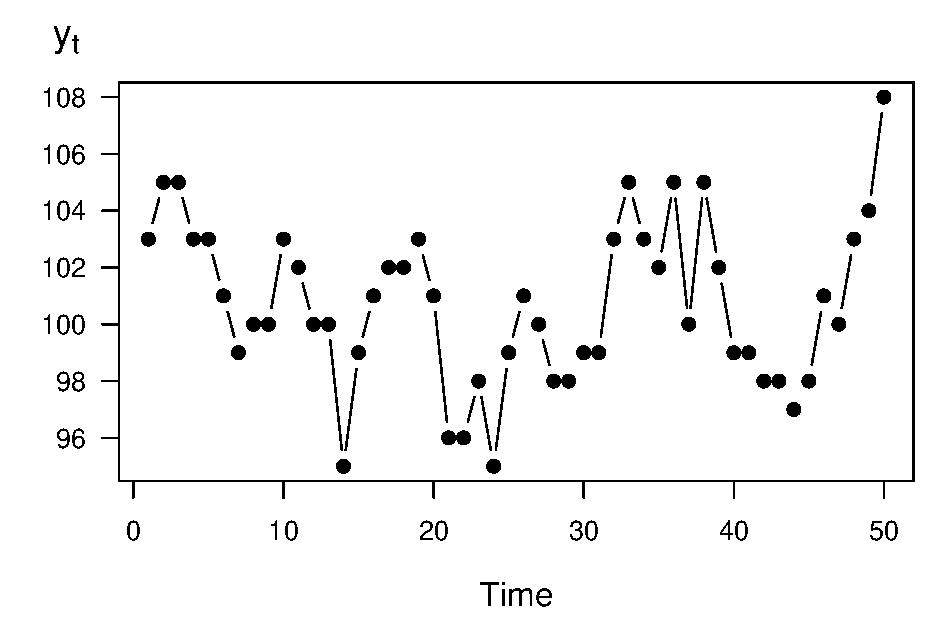
\includegraphics[width=.8\textwidth]{Chapter7Trend/RWDice.eps}
   \caption{\label{F7:RWDice} \small Time Series Plot of the Sum of Capital.}
  \end{center}
\end{figure}


The partial sums of a white noise process define a random walk
model. For example, the series $\{y_1, \ldots ,y_{50}\}$ in Figure
\ref{F7:RWDice} is a realization of the random walk model. The
phrase \emph{partial sum}\ is used because each observation, $y_t$,
was created by summing the winnings up to time $t$. For this
example, winnings, $c_t$, are a white noise process because the
amount returned, $c_t^{\ast}$, is i.i.d. In our example, your
winnings from each roll of the dice is represented using a white
noise process. Whether you win on one roll of the dice has no
influence on the outcome of the next, or previous, roll of the dice.
In contrast, your amount of capital at any roll of the dice is
highly related to the amount of capital after the next roll, or
previous roll. Your amount of capital after each roll of the dice is
represented by a random walk model.

\section{Inference using Random Walk Models}

The random walk is a commonly used time series model. To see how it
can be applied, we first discuss a few model properties. These
properties are then used to forecast and identify a series as a
random walk. Finally, this section compares the random walk to a
competitor, the linear trend in time model.

\subsubsection*{Model Properties}

To state the properties of the random walk, we first recap some
definitions. Let $c_1,\ldots ,c_T$ be $T$ observations from a white
noise process. A random walk can be expressed recursively as
\begin{equation} \label{E7:5}
y_t = y_{t-1} + c_t.
\end{equation}
By repeated substitution, we have
\begin{equation*}
y_t = c_t + y_{t-1} = c_t + \left( c_{t-1} + y_{t-2}\right) = \ldots
\end{equation*}
If we use $y_0$ to be the initial level, then we can express the
random
walk as%
\begin{equation}\label{E7:6}
y_t = y_0 + c_1 + \ldots + c_t.
\end{equation}
Equation (\ref{E7:6}) shows that a random walk is the partial sum of
a white noise process.

\marginparjed{A random walk is the partial sum of a white noise
process.}

The random walk is \emph{not} a stationary process because the
variability, and possibly the mean, depends on the time point at
which the series is observed. Taking the expectation and variance of
equation (\ref{E7:6}) yields the mean level and variability of the
random walk process:
\begin{equation*}
\mathrm{E~}y_t = y_0 + t\mu_c\text{ \ \ and \ \ }\mathrm{Var~} y_t =
t \sigma_c^2,
\end{equation*}
where $\mathrm{E~}c_t = \mu_c$\ and $\mathrm{Var~}c_t = \sigma
_c^2$. Hence, as long as there is some variability in the white
noise process ($\sigma_c^2 > 0$), the random walk is nonstationary
in the variance. Further, if $\mu_c\neq 0$, then the random walk is
nonstationary in the mean.

\marginparjed{A random walk is a nonstationary model.}

\subsubsection*{Forecasting}

How can we forecast a series of observations, $y_1,...,y_T$, that
has been identified as a realization of a random walk model? The
technique we use is to forecast the \emph{differences}, or
\emph{changes}, in the series and then sum the forecast differences
to get the forecast series. This technique is tractable because, by
the definition of a random walk model, the differences can be
represented using a white noise process, a process that we know how
to forecast.

Consider $y_{T+l}$, the value of the series $l$ lead time units into
the future. Let $c_t=y_t-y_{t-1}$ represent the differences in the
series, so that
\begin{eqnarray*}
y_{T+l} &=&y_{T+l-1}+c_{T+l} = \left( y_{T+l-2} + c_{T+l-1}\right)
+c_{T+l} = \ldots
\\
&=&y_T+c_{T+1}+ \ldots +c_{T+l}.
\end{eqnarray*}%
We interpret $y_{T+l}$ to be the current value of the series, $y_T$,
plus the partial sum of future differences.

To forecast $y_{T+l}$, because at time $T$ we know $y_T$, we need
only forecast the changes $\{c_{T+1}, \ldots, c_{T+l}\}$. Because a
forecast of a future value of a white noise process is just the
average of the process, the forecast of $c_{T+k}$ is $\overline{c}$\
for $k=1,2,\ldots,l$. Putting these together, the forecast of
$y_{T+l}$ is $y_T+l\overline{c}$ . For example, for $l=1$, we
interpret the forecast of the next value of the series to be the
current value of the series plus the average change of the series.

Using similar ideas, we have that an approximate 95\% prediction interval
for $y_{T+l}$ is%
\begin{equation*}
y_T+l\overline{c}\pm 2s_c\sqrt{l}
\end{equation*}
where $s_c$ is the standard deviation computed using the changes
$c_2,c_{3},\ldots,c_T$. Note that the width of the prediction
interval, $4 s_c \sqrt{l}$, grows as the lead time $l$ grows. This
increasing width simply reflects our diminishing ability to predict
into the future.

As an example, we rolled the dice $T=50$ times and that we would
like to forecast $y_{60}$, our sum of capital after 60 rolls. At
time 50, it turned out that our sum of money available was
$y_{50}=\$93$. Starting with $y_0 = \$100$, the average change was
$\overline{c} = -7/50 = \$-0.14$, with standard deviation
$s_c=\$2.703$. Thus, the forecast at time 60 is $93+10(-.14) =
91.6$. The corresponding 95\% prediction interval
is%
\begin{equation*}
91.6\pm 2\left( 2.703\right) \sqrt{10}=91.6\pm 17.1=\left( 74.5,108.7\right)
.
\end{equation*}

\linejed

\empexjed{LaborForcePR}\index{datasets!labor force participation
rates}

\textbf{Example: Labor Force Participation Rates.}\ecaptionjed{Labor
Force Participation Rates} Labor force participation rate ($LFPR$)
forecasts, coupled with forecasts of the population, provide us with
a picture of a nation's future workforce. This picture provides
insights to the future workings of the overall economy, and thus
$LFPR$ projections are of interest to a number of government
agencies. In the United States, $LFPR$s are projected by the Social
Security Administration, the Bureau of Labor Statistics, the
Congressional Budget Office and the Office of Management and Budget.
In the context of Social Security, policy-makers use labor force
projections to evaluate proposals for reforming the Social Security
system and to assess its future financial solvency.

A labor force participation rate is the civilian labor force divided
by the civilian noninstitutional population. These data are compiled
by the Bureau of Labor Statistics. For illustration purposes, let us
look at a specific demographic cell and show how to forecast it -
forecasts of other cells may be found in Fullerton (1999) and Frees
(2006). Specifically, we examine 1968-1998 for females, aged 20-44,
living in a household with a spouse present and at least one child
under six years of age. Figure \ref{F7:LFPR} shows the rapid
increase in $LFPR$ for this group over $T=31$\ years.


\begin{figure}[htp]
  \begin{center}
      \includegraphics[width=.8\textwidth]{Chapter7Trend/LFPR.eps}
    \caption{\label{F7:LFPR} \small Labor Force Participation Rates for Females Aged 20-44,
    Living in a Household with a Spouse Present and at least One Child under Six Years of Age.
    The plot of the series shows a rapid increase over time. Also shown are the differences which are level.}
  \end{center}
\end{figure}

\bigskip

To forecast the $LFPR$ with a random walk, we begin with our most recent
observation, $LFPR_{31}=0.6407$. We denote the change in the $LFPR$ by $%
c_t $, so that $c_t=LFPR_t-LFPR_{t-1}$. It turns out that the
average change is $\overline{c}=0.0121$ with standard deviation
$s_c=0.0101$. Thus, using a random walk model, an approximate 95\%
prediction interval for
the $l$-step forecast is%
\begin{equation*}
0.6407+0.0121l\pm \ 0.0202\sqrt{l}.
\end{equation*}%
Figure \ref{F7:LFPRFore} illustrates prediction intervals for 1999
through 2002, inclusive.

\begin{figure}[htp]
  \begin{center}
   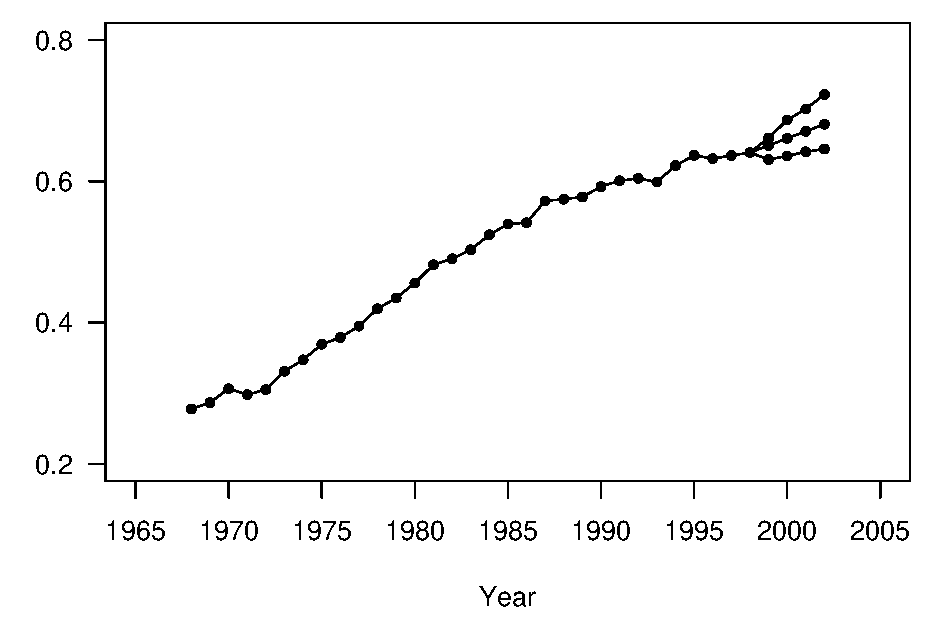
\includegraphics[width=.8\textwidth]{Chapter7Trend/LFPRFore.eps}
    \caption{\label{F7:LFPRFore} \small Time Series Plot of Labor Force Participation Rates
    with Forecast Values for 1999-2002. The middle series represent the point forecasts.
    The upper and lower series represent the upper and lower 95\% forecast intervals.
    Data for 1968-1998 represent actual values.}
  \end{center}
\end{figure}

\linejed

\subsubsection*{Identifying Stationarity}

We have seen how to do useful things, like forecasting, with random
walk models. But how do we identify a series as a realization from a
random walk? We know that the random walk is a special kind of
nonstationary model and so the first step is to examine a series and
decide whether or not it is stationary.

Stationarity quantifies the stability of a process. A process that
is strictly stationary has the same distribution over time, so we
should be able to take successive samples of modest size and show
that they have approximately the same distribution. For weak
stationary, the mean and variance are stable over time, so if one
takes successive samples of modest size, then we expect the mean
level and the variance to be roughly similar. To illustrate, when
examining time series plots, if you look at the first five, the next
five, the following five and so forth, successive samples, you
should observe approximately the same levels of averages and
standard deviations.

\marginparjed{A control chart is a time series plot with
superimposed reference lines called control limits. It is used is to
detect nonstationarity in a time series.}

\index{plots!control chart}

In quality management applications, this approach is quantified by
looking at \emph{control charts}.  A control chart is a useful
graphical device for detecting the lack of stationarity in a time
series. The basic idea is to superimpose reference lines called
\emph{control limits} on a time series plot of the data. These
reference lines help us visually detect trends in the data and
identify unusual points. The mechanics behind controls limits are
straightforward. For a given series of observations, calculate the
series mean and standard deviation, $\overline{y}$\ and $s_y$.
Define the
``upper control limit'' by $UCL=\overline{y}%
+3s_y$ and the ``lower control limit''\ by $LCL=\overline{y}-3s_y$.
Time series plots with these superimposed control limits are known
as control charts.

Sometimes the adjective \emph{retrospective} is associated with this
type of control chart. This adjective reminds the user that averages
and standard deviations are based on all the available data. In
contrast, when the control chart is used as an ongoing management
tool for detecting whether an industrial process is ``out of
control,'' a \emph{prospective control chart} may be more suitable.
Here, prospective merely means using only an early portion of the
process, that is ``in control,'' to compute the control limits.

\index{plots!Xbar chart}

A control chart that helps us to examine the stability of the mean
is the $Xbar$ chart. An $Xbar$ chart is created by combining
successive observations of modest size, taking an average over this
group, and then creating a control chart for the group averages. By
taking averages over groups, the variability associated with each
point on the chart is smaller than for a control chart for
individual observations. This allows the data analyst to get a
clearer picture of any patterns that may be evident in the mean of
the series.

\index{plots!$R$ chart}

A control chart that helps us examine the stability of the variability is
the $R$ chart. As with the $Xbar$ chart, we begin by forming successive
groups of modest size. With the $R$ chart, for each group we compute the
range, which is the largest minus the smallest observation, and then create
a control chart for the group ranges. The range is a measure of variability
that is simple to compute, an important advantage in manufacturing
applications.

\subsubsection*{Identifying Random Walks}

Suppose that you suspect that a series is nonstationary, how do
identify the fact that these are realizations of a random walk
model? Recall that the expected value of a random walk,
$\mathrm{E~}y_t=y_0+t\mu_c$, suggests that such a series follows a
linear trend in time. The variance of a random walk,
$\mathrm{Var~}y_t=t\sigma_c^2$, suggests that the variability of a
series gets larger as time $t$ gets large. First, a control chart
can help us to detect these patterns, whether they are of a linear
trend in time, increasing variability, or both.

\marginparjed{If the original data follows a random walk model, then
the differenced series follows a white noise process model.}

Second, if the original data follows a random walk model, then the
differenced series follows a white noise process model. If a random walk
model is a candidate model, you should examine the differences of the
series. In this case, the time series plot of the differences should be a
stationary, white noise process that displays no apparent patterns. Control
charts can help us to detect this lack of patterns.

Third, compare the standard deviations of the original series and
the differenced series. We expect the standard deviation of the
original series to be greater than the standard deviation of the
differenced series. Thus, if the series can be represented by a
random walk, we expect a substantial reduction in the standard
deviation when taking differences.

\linejed

\index{datasets!labor force participation rates}

\textbf{Example: Labor Force Participation Rates - Continued.} In
Figure \ref{F7:LFPR}, the series displays a clear upward trend
whereas the differences show no apparent trends over time. Further,
when computing differences of each series, it turned out
that%
\begin{equation*}
0.1197=SD(series)>SD(differences)=0.0101.
\end{equation*}
Thus, it seems reasonable to tentatively use a random walk as a
model of the labor force participation rate series.

In Chapter 8, we will discuss two additional identification devices.
These are scatter plots of the series versus a lagged version of the
series and the corresponding summary statistics called
\emph{autocorrelations}.

 \linejed
\subsubsection*{Random Walk versus Linear Trend in Time Models}

The labor force participation rate example could be represented
using either a random walk or a linear trend in time model. These
two models are more closely related to one another than is evident
at first glance. To see this relationship, recall that the linear
trend in time model can be written as
\begin{equation}\label{E7:7}
y_t = \beta_0 + \beta_1 t + \varepsilon_t,
\end{equation}
where $\{\varepsilon_t\}$ is a white noise process. If $\{y_t\}$ is
a random walk, then it can be modeled as a partial sum as in
equation (\ref{E7:6}). We can also decompose the white noise process
into a mean $\mu _c$ plus another white noise process, that is, $c_t
= \mu_c + \varepsilon_t$. Combining these two ideas, a random walk
model can be written as

\begin{equation} \label{E7:8}
y_t = y_0 + \mu_c t + u_t
\end{equation}
where $u_t = \sum_{j=1}^{t} \varepsilon_j$. Comparing equations
(\ref{E7:7}) and (\ref{E7:8}), we see that the two models are
similar in that the deterministic portion is a linear function of
time. The difference is in the error component. The error component
for the linear trend in time model is a stationary, white noise
process. The error component for the random walk model is
nonstationary because it is the partial sum of white noise
processes. That is, the error component is also a random walk. Many
introductory treatments of the random walk model focus on the ``fair
game'' example and ignore the drift term $\mu_c$. This is
unfortunate because the comparison between the random walk model and
the linear trend in time model is not as clear when the parameter
$\mu_c$ is equal to zero.

\section{Filtering to Achieve Stationarity}


A \emph{filter} is a procedure for reducing observations to white
noise. In regression, we accomplished this by simply subtracting the
regression function from the observations, that is, $y_i - (\beta_0
+ \beta_1 x_{1i} + \ldots + \beta_k x_{ki})=\varepsilon_i$.
Transformation of the data is another device for filtering that we
introduced in Chapter 1 when analyzing cross-sectional data. We
encountered another example of a filter in Section
\ref{S7:RandomWalk}. There, by taking differences of observations,
we reduced a random walk series to a white noise process.

\marginparjed{A filter is a procedure for reducing observations to
white noise.}\index{time series terms and concepts!filter}

An important theme of this text is to use an iterative approach for
fitting models to data. In particular, in this chapter we discuss
techniques for reducing a sequence of observations to a stationary
series. By definition, a stationary series is stable and hence is
far easier to forecast than an unstable series. This stage,
sometimes known as \emph{pre-processing} the data, generally
accounts for the most important sources of trends in the data. The
next chapter will present models that account for subtler trends in
the data.

\subsubsection*{Transformations}

When analyzing longitudinal data, transformation is an important
tool used to filter a data set. Specifically, using a logarithmic
transformation tends to shrink ``spread out'' data. This feature
gives us an alternative method to deal with a process where the
variability appears to grow with time. Recall the first option
discussed is to posit a random walk model and examine differences of
the data. Alternatively, one may take a logarithmic transform that
helps to reduce increasing variance through time.

Further, from the random walk discussion, we know that if both the
series variance and log series variance increase through time, the
differences of the log transform might handle this increasing
variability. Differences of natural logarithms are particularly
pleasing because they can be interpreted as \emph{proportional
changes}. To see this, define $pchange_t=(y_t/y_{t-1})-1$. Then,
\begin{equation*}
\ln y_t-\ln y_{t-1} = \ln \left( \frac{y_t}{y_{t-1}}\right) = \ln
\left( 1+pchange_t\right) \approx pchange_t.
\end{equation*}
Here we use the Taylor series approximation $\ln (1+x) \approx x$
that is appropriate for small values of $|x|$.

\linejed

\index{datasets!Standard and Poor's quarterly index}

\textbf{Example: Standard and Poor's Composite Quarterly
Index.}\ecaptionjed{Standard and Poor's Composite Quarterly Index}
An important task of a financial analyst is to quantify costs
associated with future cash flows. We consider here funds invested
in a standard measure of overall market performance, the Standard
and Poor's (S\&P) 500 Composite Index. The goal is to forecast the
performance of the portfolio for discounting of cash flows.

In particular, we examine the S\&P Composite Quarterly Index for the
years 1936 to 2007, inclusive. By today's standards, this period may
not be the most representative because the Depression of the 1930's
is included. The motivation to analyze these data is from the
Institute of Actuaries ``Report of the Maturity Guarantees Working
Party'' (1980) who analyzed the series from 1936 to 1977, inclusive.
This paper studied the long term behavior of investment returns from
an actuarial viewpoint. We complement that work by showing how
graphical techniques can suggest a useful transformation for
reducing the data to a stationary process.

The data are shown in Figure \ref{F7:SandPTS}. From the original
index values in the upper left-hand panel, we see that the mean
level and variability increases with time. This pattern clearly
indicates that the series is nonstationary.

From our discussions in Sections \ref{S7:Trends} and
\ref{S7:RandomWalk}, a candidate model that has these properties is
the random walk. However, the time series plot of the differences,
in upper right-hand panel of Figure \ref{F7:SandPTS}, still
indicates a pattern of variability increasing with time. The
differences are not a white noise process so the random walk is not
a suitable model for the S \& P 500 Index.

An alternative transformation is to consider logarithmic values of
the series. The time series plot of logged values, presented in
lower left-hand panel of Figure \ref{F7:SandPTS}, indicates the the
mean level of the series increases over time and is not level. Thus,
the logarithmic index is not stationary.

Yet another approach is to examine differences of the logarithmic
series. This is especially desirable when looking at indices, or
\textquotedblleft breadbaskets,\textquotedblright\ because the
difference of logarithms can be interpreted as proportional changes.
From the final time series plot, in the lower right-hand panel of
Figure \ref{F7:SandPTS}, we see that there are fewer discernible
patterns in the transformed series, the difference of logs. This
transformed series seems to be stationary. It is interesting to note
that there seems to be a higher level of volatility at the beginning
of the series. This type of changing volatility is more difficult to
model and has recently been the subject of considerable attention in
the financial economics literature (see, for example, Hardy, 2003).


\begin{figure}[htp]
  \begin{center}
    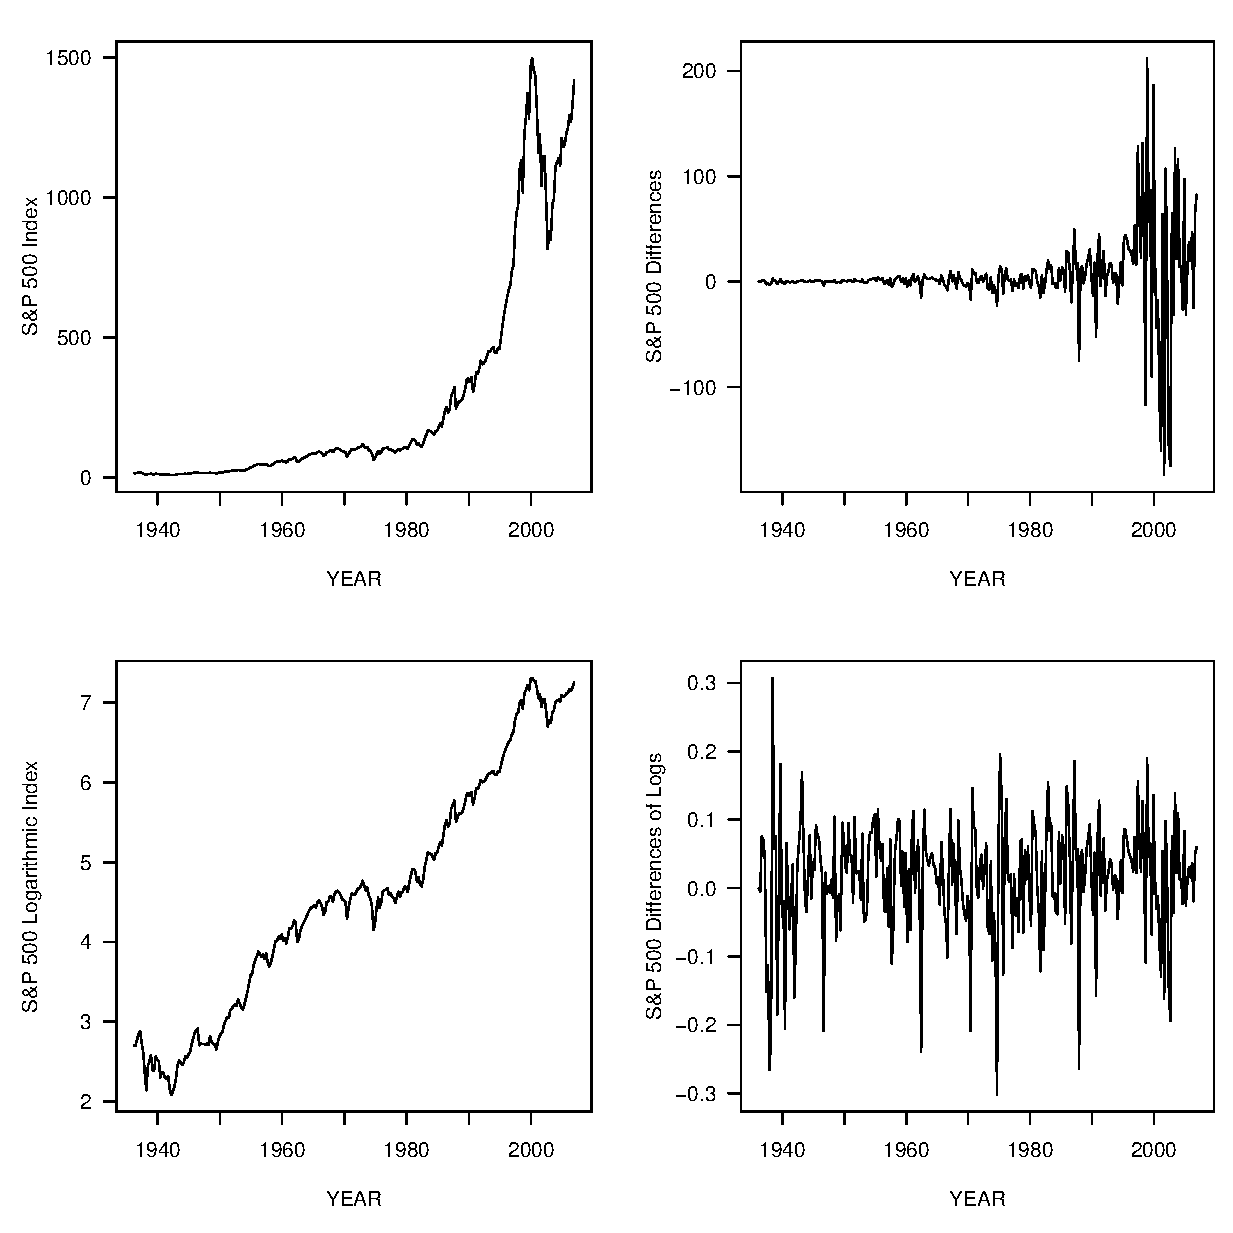
\includegraphics[width=1\textwidth]{Chapter7Trend/SandPTS.eps}
    \caption{\label{F7:SandPTS} \small Time Series Plots of the S \& P 500 Index. The upper
left-hand panel shows the original series that is nonstationary in
the mean and in the variability. The upper right-hand panel shows
the differences in the series that is nonstationary in the
variability. The lower left-hand panel shows the logarithmic index
that is nonstationary in the mean. The lower right hand panel shows
the differences of the logarithmic index that appears to be
stationary in the mean and in the variability.}
  \end{center}
\end{figure}

\linejed

\section{Forecast Evaluation}

Judging the accuracy of forecasts is important when modeling time series
data. In this section, we present forecast evaluation techniques that:

\begin{itemize}
\item Help detect recent unanticipated trends or patterns in the data.

\item Are useful for comparing different forecasting methods.

\item Provide an intuitive and easy to explain method for evaluating the
accuracy of forecasts.
\end{itemize}

In the first five sections of Chapter 7, we presented several techniques for
detecting patterns in residuals from a fitted model. Measures that summarize
the distribution of residuals are called \emph{goodness-of-fit statistics}.
As we saw in our study of cross-sectional models, by fitting several
different models to a data set, we introduce the possibility of overfitting
the data. To address this concern, we will use \emph{out-of-sample validation%
} techniques, similar to those introduced in Section 6.5.

To perform an out-of-sample validation of a proposed model, ideally
one would develop the model on a data set and then corroborate the
model's usefulness on a second, independent data set. Because two
such ideal data sets are rarely available, in practice we can split
a data set into two subsamples, a \emph{model development subsample}
and a \emph{validation subsample}. For longitudinal data, the
practice is to use the beginning part of the series, the first $T_1$
observations, to develop one or more candidate models. The latter
part of the series, the last $T_2=T-T_1$ observations, are used to
evaluate the forecasts. For example, we might have ten years of
monthly data so that $T=120$. It would be reasonable to use the
first eight years of data to develop a model and the last two years
of data for validation, yielding $T_1=96$ and $T_2=24$.

Thus, observations $y_1,\ldots , y_{T_1}$ are used to develop a
model. From these $T_1$ observations, we can determine the
parameters of the candidate model. Using the fitted model, we can
determine fitted values for the model validation subsample for $t =
T_1 + 1,T_1+2, \ldots, T_1+T_2$. Taking the difference between the
actual and fitted values yield one-step forecast residuals, denoted
by $e_t=y_t-\widehat{y}_t$. These forecast residuals are the basic
quantities that we will use to evaluate and compare forecasting
techniques.

To compare models, we use a four-step process similar to that described in
Section 6.5, described as follows.

\boxedjed

\textit{Out-of-Sample Validation Process}

\begin{compactenum}[1.]
\item Divide the sample of size $T$ into two subsamples, a model development
subsample ($t=1,\ldots,T_1$) and a model validation subsample
($t=T_1+1, \ldots, T_1 + T_2$).

\item Using the model development subsample, fit a candidate model to the
data set $t=1,\ldots,T_1$.

\item Using the model created in Step 2 and the dependent variables up to
and including $t-1$, forecast the dependent variable
$\widehat{y}_t$, where $t=T_1+1, \ldots, T_1+T_2$.

\item Use actual observations and the fitted values computed in Step 3 to
compute one-step forecast residuals, $e_t = y_t- \widehat{y}_t$, for
the model validation subsample. Summarize these residuals with one
or more comparison statistics, described below.
\end{compactenum}

Repeat Steps 2 through 4 for each of the candidate models. Choose
the model with the smallest set of comparison statistics.


\end{boxedminipage}

\bigskip

Out-of-sample validation can be used to compare the accuracy of forecasts
from virtually any forecasting model. As we saw in Section 6.5, we are not
limited to comparisons where one model is a subset of another, where the
competing models use the same units for the response, and so on.

There are several statistics that are commonly used to compare
forecasts.

\boxedjed

\textit{Commonly Used Statistics for Comparing Forecasts}

1. The \emph{mean error statistic}, defined by%
\begin{equation*}
ME=\frac{1}{T_2}\sum_{t=T_1+1}^{T_1+T_2}e_t.
\end{equation*}
This statistic measures recent trends that are not anticipated by the model.

2. The \emph{mean percent error}, defined by
\begin{equation*}
MPE=\frac{100}{T_2}\sum_{t=T_1+1}^{T_1+T_2}\frac{e_t}{y_t}.
\end{equation*}
This statistic is also a measure of trend, but examines error relative to
the actual value.

3. The \emph{mean square error}, defined by%
\begin{equation*}
MSE=\frac{1}{T_2}\sum_{t=T_1+1}^{T_1+T_2}e_t^2.
\end{equation*}
This statistic can detect more patterns than $ME$. It is the same as
the cross-sectional $SSPE$ statistic, except for the division by
$T_2$.

4. The \emph{mean absolute error}, defined by
\begin{equation*}
MAE=\frac{1}{T_2}\sum_{t=T_1+1}^{T_1+T_2}|e_t|.
\end{equation*}
Like $MSE$, this statistic can detect more than trend patterns than $ME$.
The units of $MAE$ are the same as the dependent variable.

5. The \emph{mean absolute percent error}, defined by%
\begin{equation*}
MAPE=\frac{100}{T_2}\sum_{t=T_1+1}^{T_1+T_2}|\frac{e_t}{y_t}|.
\end{equation*}%
Like $MAE$, this statistic can detect more than trend patterns. Like $MPE$,
it examines error relative to the actual value.

\end{boxedminipage}

\bigskip

\linejed

\index{datasets!labor force participation rates}

\textbf{Example: Labor Force Participation Rates - Continued. }We
can use out-of-sample validation measures to compare two models for
the $LFPR$s; the linear trend in time model and the random walk
model. For this illustration, we examined the labor rates for years
1968 through 1994, inclusive. This corresponds to $T_1 = 27$
observations defined in Step 1. Data were subsequently gathered on
rates for 1995 through 1998, inclusive, corresponding to $T_2 = 4$
for out-of-sample validation. For Step 2, we fit each model using
$t=1,\ldots,27$, earlier in this chapter. For Step 3, the one-step
forecasts are:

\begin{equation*}
\widehat{y}_t = 0.2574 + 0.0145t
\end{equation*}%
and%
\begin{equation*}
\widehat{y}_t = y_{t-1} + 0.0132
\end{equation*}
for the linear trend in time and the random walk models,
respectively. For Step 4, Table \ref{T7:ForecastComparison}
summarizes the forecast comparison statistics. Based on these
statistics, the choice of the model is clearly the random walk.

\scalefont{0.9}
\begin{table}[h]
\caption{\label{T7:ForecastComparison} Out of Sample Forecast
Comparison}
\begin{center}
\begin{tabular}{c|ccccc}
\hline & $ME$ & $MPE$ & $MSE$ & $MAE$ & $MAPE$ \\ \hline
\multicolumn{1}{l|}{Linear trend in time model} & -0.0488 & -0.0766
& 0.0026
& 0.0488 & 0.0766 \\
\multicolumn{1}{l|}{Random walk model} & -0.0007 & ~0.0012 & 0.0001
& 0.0115 & 0.0180 \\ \hline
\end{tabular}\end{center}\end{table}
\scalefont{1.1111}

\linejed



\section{Further Reading and References}

For many years, actuaries in North America were introduced to time
series analysis from Miller and Wichern (1977), Abraham and Ledolter
(1983) and Pindyck and Rubinfeld (1991). A more recent book-long
introduction is Diebold (2004). Diebold contains a brief
introduction to regime-switching models.


Because of the difficulties regarding their specification and
limited forecasting use, we do not explore causal models further in
this text. For more details on causal models, the interested reader
is referred to Pindyck and Rubinfeld (1991).

\bigskip

\textbf{Chapter References}

\begin{multicols}{2}

\scalefont{0.9}


``Report of the Maturity Guarantees Working Party'' (1980).
\textit{Journal of the Institute of Actuaries} 107, pp. 103-213.

Abraham, Bovas and  Johannes Ledolter (1983). \textit{Statistical
Methods for Forecasting}. John Wiley \& Sons, New York.

Diebold, Francis X. (2004). \textit{Elements of Forecasting}, Third
Edition. Thompson South-Western, Mason, OH.

Frees, Edward W. (2006). Forecasting of labor force participation
rates. \emph{The Journal of Official Statistics} 22(3), 453-485.

Fullerton, Howard N., Jr. (1999). Labor force projections to 2008:
steady growth and changing composition. \textit{Monthly Labor
Review}, November, pp. 19-32.

Granger, Clive W. J and P. Newbold (1974). Spurious regressions in
econometrics. \textit{Journal of Econometrics} 2, 111-120.

Hardy, Mary (2001). A regime-switching model of long-term stock
returns. \emph{North American Actuarial Journal} 5(2), 41-53.

Hardy, Mary (2003). \emph{Investment Guarantees: Modeling and Risk
Management for Equity-Linked Life Insurance}. John Wiley \& Sons,
New York.

Miller, Robert B. and Dean W. Wichern (1977). \emph{Intermediate
Business Statistics: Analysis of Variance, Regression and Time
Series}. Holt, Rinehart and Winston, New York.

Pindyck, R.S. and D.L. Rubinfeld (1991). \textit{Econometric Models
and Economic Forecasts,} Third Edition, McGraw-Hill, New York.

\scalefont{1.1111}

\end{multicols}

\section{Exercises}

\scalefont{0.90}
\begin{exercises}

\item Consider a random walk $\{y_t \}$ as the partial sum of a white noise process $\{ c_t \}$ with
mean $\mathrm{E}~c_t= \mu_c$ and variance $\mathrm{Var}~c_t =
\sigma_c^2$. Use equation (\ref{E7:6}) to show

a.  $\mathrm{E}~y_t= y_0 + t \mu_c$, where $y_0$ is the initial
value and

b.  $\mathrm{Var}~y_t= t \sigma_c^2$.

\item Consider a random walk $\{y_t \}$ as the partial sum of a white noise process $\{ c_t
\}$.

a. Show that the $l$-step forecast error is
$y_{T+l}-\widehat{y_{T+l}} = \sum_{j=1}^l (c_{T+j} - \bar{c} ).$

b. Show that the approximate variance of the $l$-step forecast error
is $l \sigma_c^2.$



\empexjed{EuroExchange}\index{datasets!Euro exchange rates}

\item \textbf{Euro Exchange Rates}. The exchange rate that we consider is the amount of Euros that one
can purchase for one US dollar. We have $T=699$ daily observations
from the period April 1, 2005 through January 8, 2008. These data
were obtained from the Federal Reserve (H10 report). \emph{Source}:
Federal Reserve Bank of New York. Note: The data are based on noon
buying rates in New York from a sample of market participants and
they represent rates set for cable transfers payable in the listed
currencies. These are also the exchange rates required by the
Securities and Exchange Commission for the integrated disclosure
system for foreign private issuers.


\begin{figure}[htp]
  \begin{center}
   \includegraphics[width=1\textwidth,angle=0,scale=0.6]{Chapter7Trend/EuroPlot1.eps}
   \caption{\label{Ex:EuroPlot1} \small Time series plot of the Euro exchange rate.}
  \end{center}
\end{figure}


a. Figure \ref{Ex:EuroPlot1} is a time series plot of the Euro
exchange rate.

a(i). Define the concept of a stationary time series.

a(ii). Is the EURO series stationary? Use your definition in part
a(i) to justify your response.

b. Based on an inspection of Figure \ref{Ex:EuroPlot1} in part (a),
you decide to fit a quadratic trend model of the data. Figure
\ref{Ex:EuroPlot2} superimposes the fitted value on a plot of the
series.


\begin{figure}[htp]
  \begin{center}
   \includegraphics[width=1\textwidth,angle=0,scale=0.6]{Chapter7Trend/EuroPlot2.eps}
   \caption{\label{Ex:EuroPlot2} \small  Quadratic fitted curve superimposed on the Euro exchange rate.}
  \end{center}
\end{figure}

b(i). Cite several basic regression statistics that summarize the
quality of the fit.

b(ii). Briefly describe any residual patterns that you observe in
Figure \ref{Ex:EuroPlot2}.

b(iii). Here, TIME varies from $1, 2, \ldots, 699$. Using this model
calculate the three-step forecast corresponding to TIME = 702.


\bigskip

c. To investigate a different approach, DIFFEURO, calculate the
difference of EURO. You decide to model DIFFEURO as a white noise
process.

c(i).  What is the name for the corresponding model of EURO?

c(ii). The most recent value of EURO is $EURO_{699} = 0.6795$. Using
the model identified in part c(i), provide a three-step forecast
corresponding to TIME = 702.

c(iii).  Using the model identified in part c(i) and the point
forecast in part c(ii), provide the corresponding 95\% prediction
interval for $EURO_{702}$.



\end{exercises}
\scalefont{1.1111}
